\chapter{Project management}
\label{chap:project-management}

\defaultInstructions

\begin{length}
There are no strict length requirements for this chapter.  However, it is important that the writing is clear and concise.  Avoid repeating yourself.  Make sure to clearly signpost evidence for claims.  It should be possible for a reader to understand this chapter without consulting other sources.  It is expected that a typical project needs 3--6 pages, but this can vary considerably from project to project.
\end{length}

\begin{expectations}
In this chapter, the team must present, reflect on, and evaluate the team's approaches to project management.  This discussion should present the main approaches to project management the team decided to use.  Include the team's rationale for these decisions, and the team's observations on the effectiveness of each approach.

During the project, the team may have made significant changes to project management approaches, or made new decisions where initial arrangements were insufficient.  A typical team will also have encountered difficulties, such as risks that materialised and impacted the team.  Discuss the most critical decisions the team made, why you made them, and what the results were.  If certain approaches were not entirely successful, discuss what you would do differently in a future project.  

A good report shows a systematic approach to project management, justifications for key decisions, and a critical reflection on the effectiveness of different approaches.  Ideally, the justifications and reflections in this chapter are based on project management theory.

Note that ``a systematic approach to project management'', ``critical reflection'', and use of ``project management theory'' do not necessary imply that your team's project management approach is a success story.  Thoughful, considered project management improves your chances of success, but projects do not always go according to plan and team's make mistakes.  The markers are looking for 
\begin{itemize}
    \item Good justifications for approaching a project in a particular way.
    \item Critical reflection on the results, including recognition of problems.
    \item The team taking ownership of the problems they encountered.
\end{itemize}

There is no one best way of organising this content.  One approach is to cover different phases of the project management lifecycle (from initialisation to project close).  Another approach is to cover different project management tasks (e.g. team management, scheduling, planning, risk, etc.).  Yet another approach is to cover the most impactful events.  Each project is different and you should take the approach that works best for your team.

There is also no minimum or maximum number of issues to cover.  Cover what is more important in the depth necessary to do the topic justice.
\end{expectations}

\subsection{Project Overview and Scope}
During initiation, we formally agreed on the project scope as captured in our scope statement. The primary outcome of this phase was to gain clarity on what our application would and would not include. We found this step highly effective at allowing us to understand the true value we want to provide, which allowed us to implement features that are coherent and make sense. Identifying stakeholders early was also key to gain clarity on who we are providing value to. Below are some of the key decisions made during our first two project initiation meetings in week 1.

\subsubsection{Project Purpose and Description}
A mobile-web hybrid application that provides a flexible way for users to track their habits. The app will help users enforce new good habits and assist with ending bad habits. By offering clear data visualisations, a user-friendly interface, and customisable habits, the system helps users manage their goals.

\subsubsection{Desired Results and Exclusions}
\textbf{In Scope:}
\begin{itemize}
    \item Building a habit and activity tracking app using React Native with Expo Go, TypeScript/JavaScript, and a MySQL database.
    \item Allowing users to register/log in, set custom habit goals, and track progress.
    \item Providing clear data visualisations (charts, graphs, analytics) and a data export feature.
\end{itemize}

\textbf{Exclusions:}
\begin{itemize}
    \item Multi-platform support is not a priority.
    \item Frequent reminders or push notifications are out of scope; notifications will be weekly.
    \item Direct integration with third-party apps/services.
\end{itemize}

\subsubsection{Constraints}
\textbf{Time:} The project must be completed within a 10-week window (13/01/25 – 27/03/25).\\
\textbf{Team Size:} There are 9 group members, requiring effective communication to manage coordination.\\
\textbf{Skill Sets:} The team’s familiarity with React Native, Expo Go, TypeScript, and MySQL may limit feature complexity.\\
\textbf{Workload Balance:} The team must juggle other academic responsibilities alongside this development project.

\subsection{Stakeholder Identification}
We used the D.A.N.C.E. framework to classify stakeholders, as detailed in Chapter 2 of this report. At this stage, we focused on:
\begin{itemize}
    \item \textbf{Primary Users} - those who directly interact with the app.
    \item \textbf{Development Team} - responsible for planning, designing, building, and deployment.
    \item \textbf{Academic Supervisors} - providing guidance and evaluation.
\end{itemize}

\subsection{Our Project Management Approach}
Initially, we agreed to combine Agile techniques (e.g., using Trello with story points) with a more traditional Waterfall Model (e.g., a fixed final deadline, staged deliverables). This hybrid approach provided us with:
\begin{itemize}
    \item Flexibility to reprioritise features when faced with new insights or changing team availability.
    \item Structure to ensure mandatory deliverables (e.g., report chapters, final submission) meet set deadlines.
\end{itemize}

\section{Planning}
Planning was critical in laying out how we would achieve the objectives defined in our scope statement. As recommended by project management theory (PMBOK, 2017), we focused on risk management, scheduling, and communication planning.

\subsection{Risk Management}
We identified potential risks early on and agreed on their probability and impact. Identifying risks early allowed us to understand how to quickly minimise problems when they would inevitably arise, helping us waste less time. For example, as seen in Table 4.1., one risk we identified was "Missed deadlines" which led us to understand the importance of setting weekly task deadlines.

\begin{table}[H]
    \centering
    \caption{Project Risk Management (source: Team Feedback Meeting Minutes 29/01/25)}
    \label{table:project_risk}
    \begin{tabular}{|p{5cm}|c|c|p{6cm}|}
        \hline
        \textbf{Risk} & \textbf{Probability} & \textbf{Impact} & \textbf{Mitigation} \\
        \hline
        Poor team communication & Medium & High & Establish a weekly meeting date (Wednesdays) and communicate regularly using Discord. \\
        \hline
        Missed deadlines & Medium & High & Use Trello regularly, assign deadlines to each task, and keep the group updated. \\
        \hline
        Deployment and Hosting issues & Low & High & Choose a reliable hosting provider. Test deployment. \\
        \hline
        Delays caused by dependencies in code development & Medium & High & Assign tasks thoughtfully and keep the group updated with tasks. \\
        \hline
        Technical issues & Medium & High & Make sure to test regularly. Regular communication with the team. \\
        \hline
    \end{tabular}
\end{table}

We also re-evaluated risks during the project review meeting, which was effective at helping us identify where we were falling behind as a team, such as security issues (see Figure \ref{fig:reeval_risks}). (See Section \ref{sec:project_review} for the evaluation of our project review meeting).

\begin{figure}[H]
    \centering
    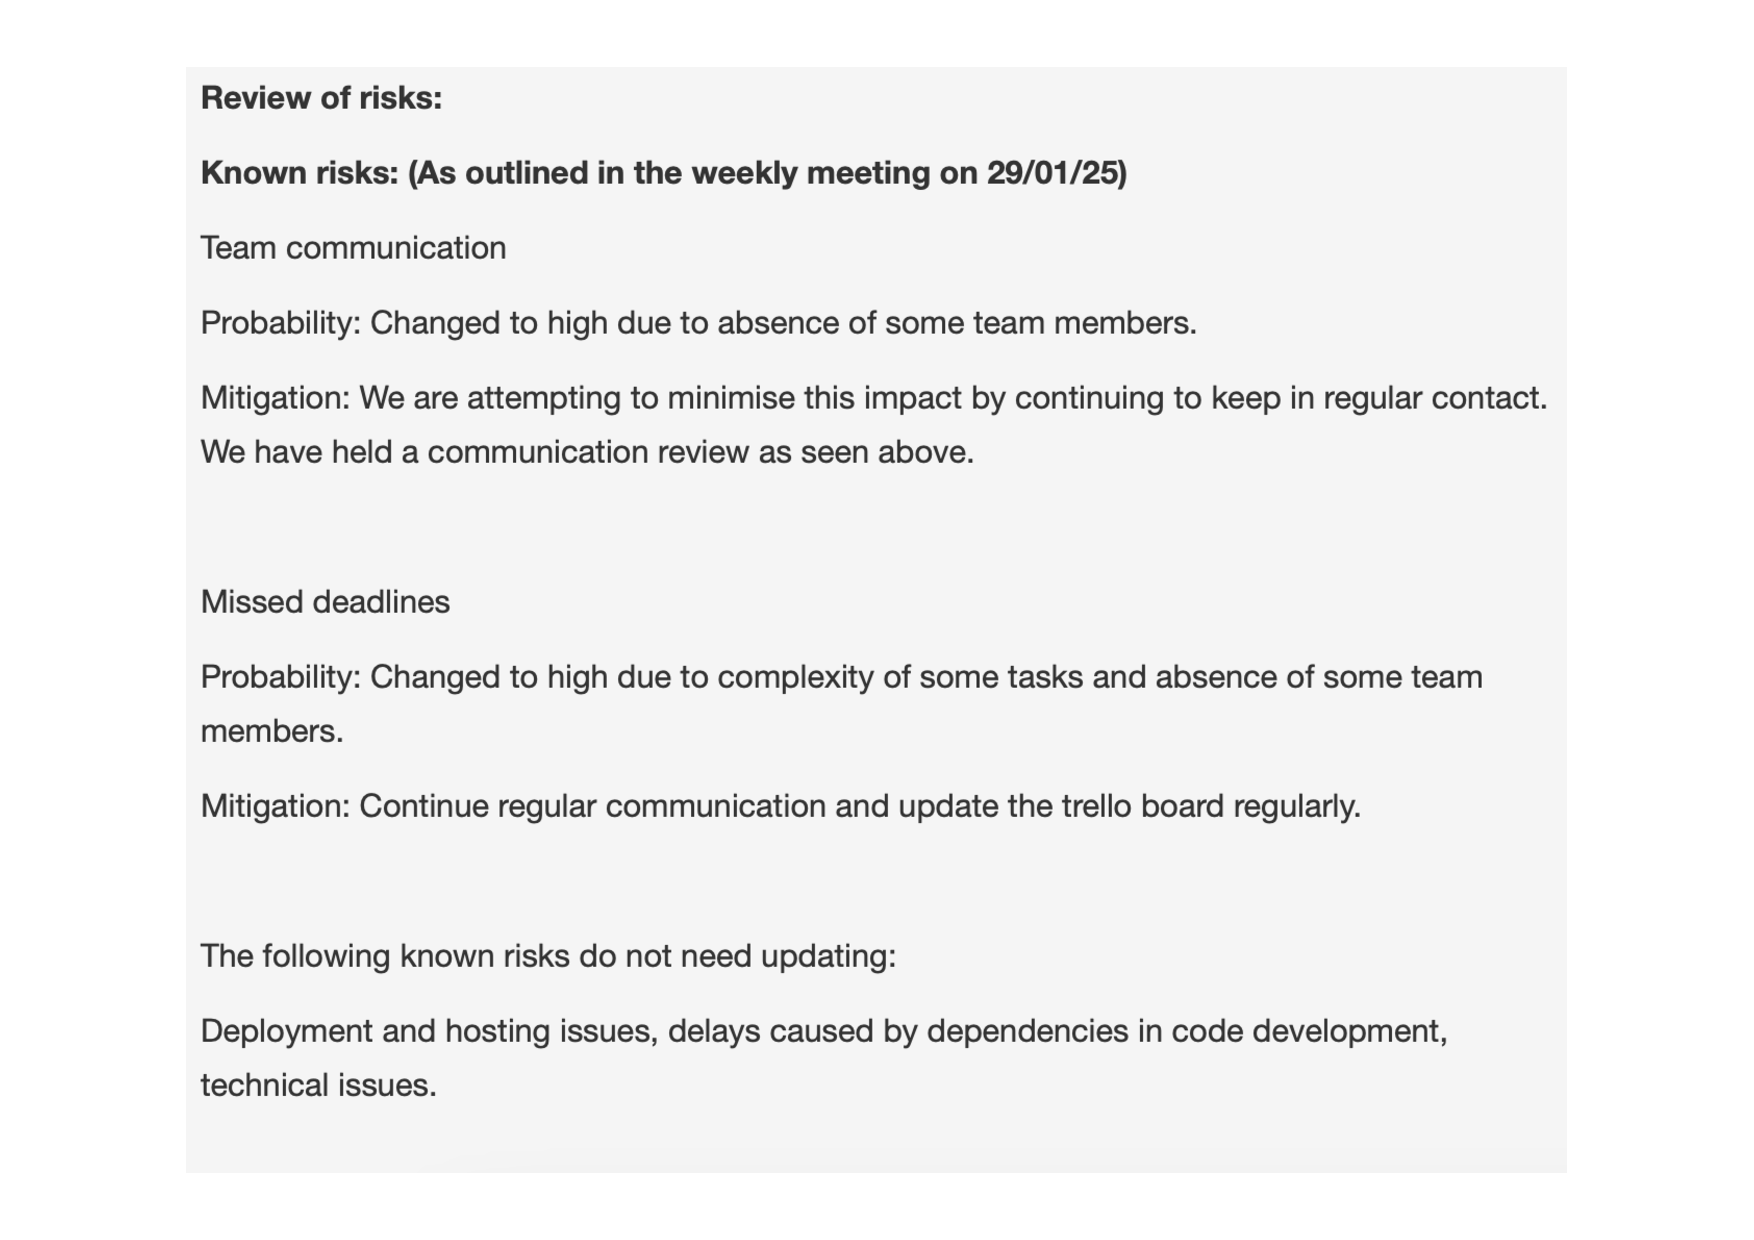
\includegraphics[width=0.7\textwidth]{resources/risk_review.pdf}
    \caption{Reevaluation of Risks (source: Team Feedback Meeting Minutes 26/02/25)}
    \label{fig:reeval_risks}
\end{figure}

\subsection{Scheduling}
Our scheduling used Trello to break down epics into manageable tasks. We assigned story points on a scale of 1 to 5. This allowed us to:
\begin{itemize}
    \item Estimate the project velocity (around 15 story points/week during our project review meeting).
    \item Track our backlog of tasks and ensure we were on track for submission by the deadline.
\end{itemize}

\begin{figure}[H]
    \centering
    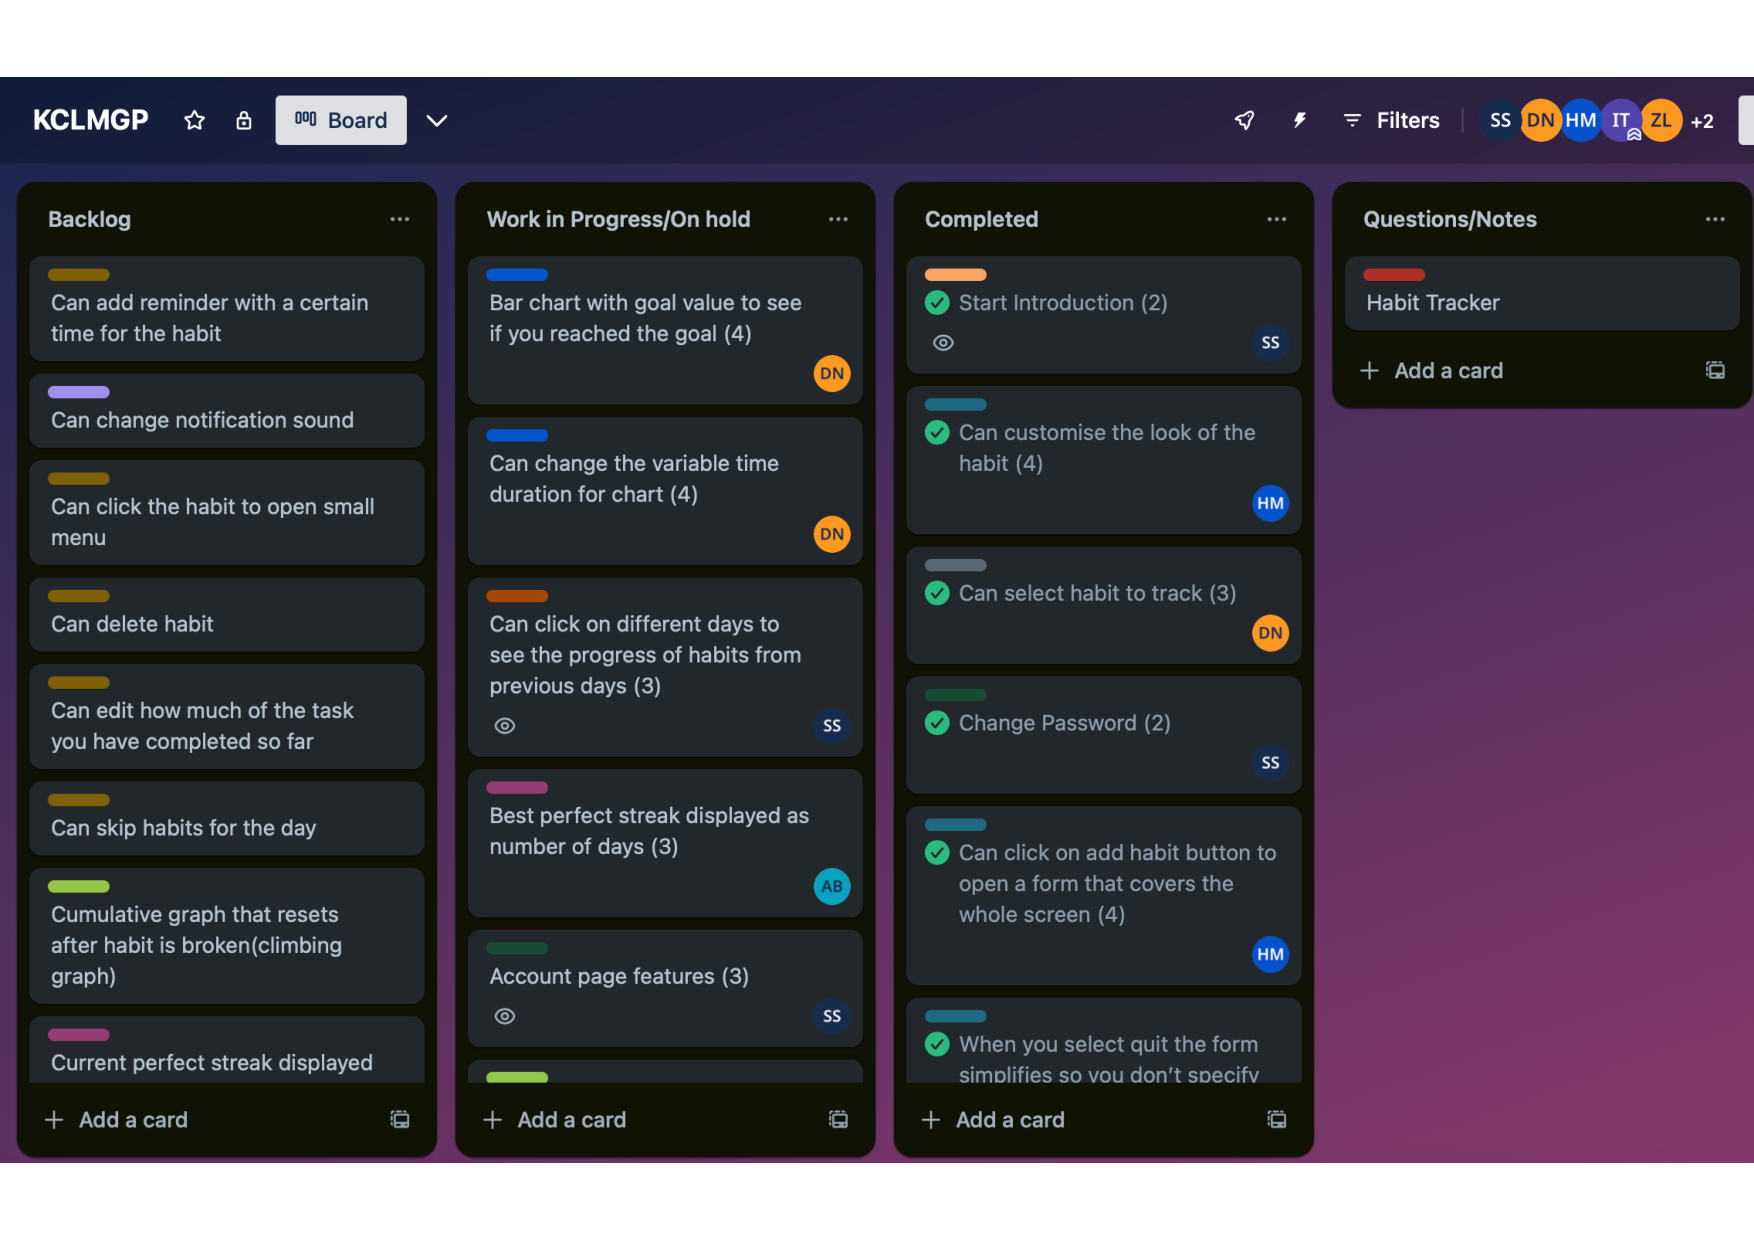
\includegraphics[width=0.7\textwidth]{resources/trello_board.pdf}
    \caption{Screenshot of Trello board showing tasks and progress}
    \label{fig:trello_tasks}
\end{figure}

As seen in Figure \ref{fig:trello_tasks}, one improvement we identified was the need to include a ‘Testing’ section on our Trello board. This would have ensured that all tasks marked as ‘complete’ were thoroughly tested beforehand, preventing bugs and the need for retrospective testing.

Another aspect that worked well was using color-coded labels for each task (see Figure \ref{fig:trello_tasks}), which allowed us to separate different areas of our app. This helped organize task allocation and reduced dependencies in code development, which addressed one of our ‘High’ impact risks (see Table \ref{table:project_risk}).

\begin{figure}[H]
    \centering
    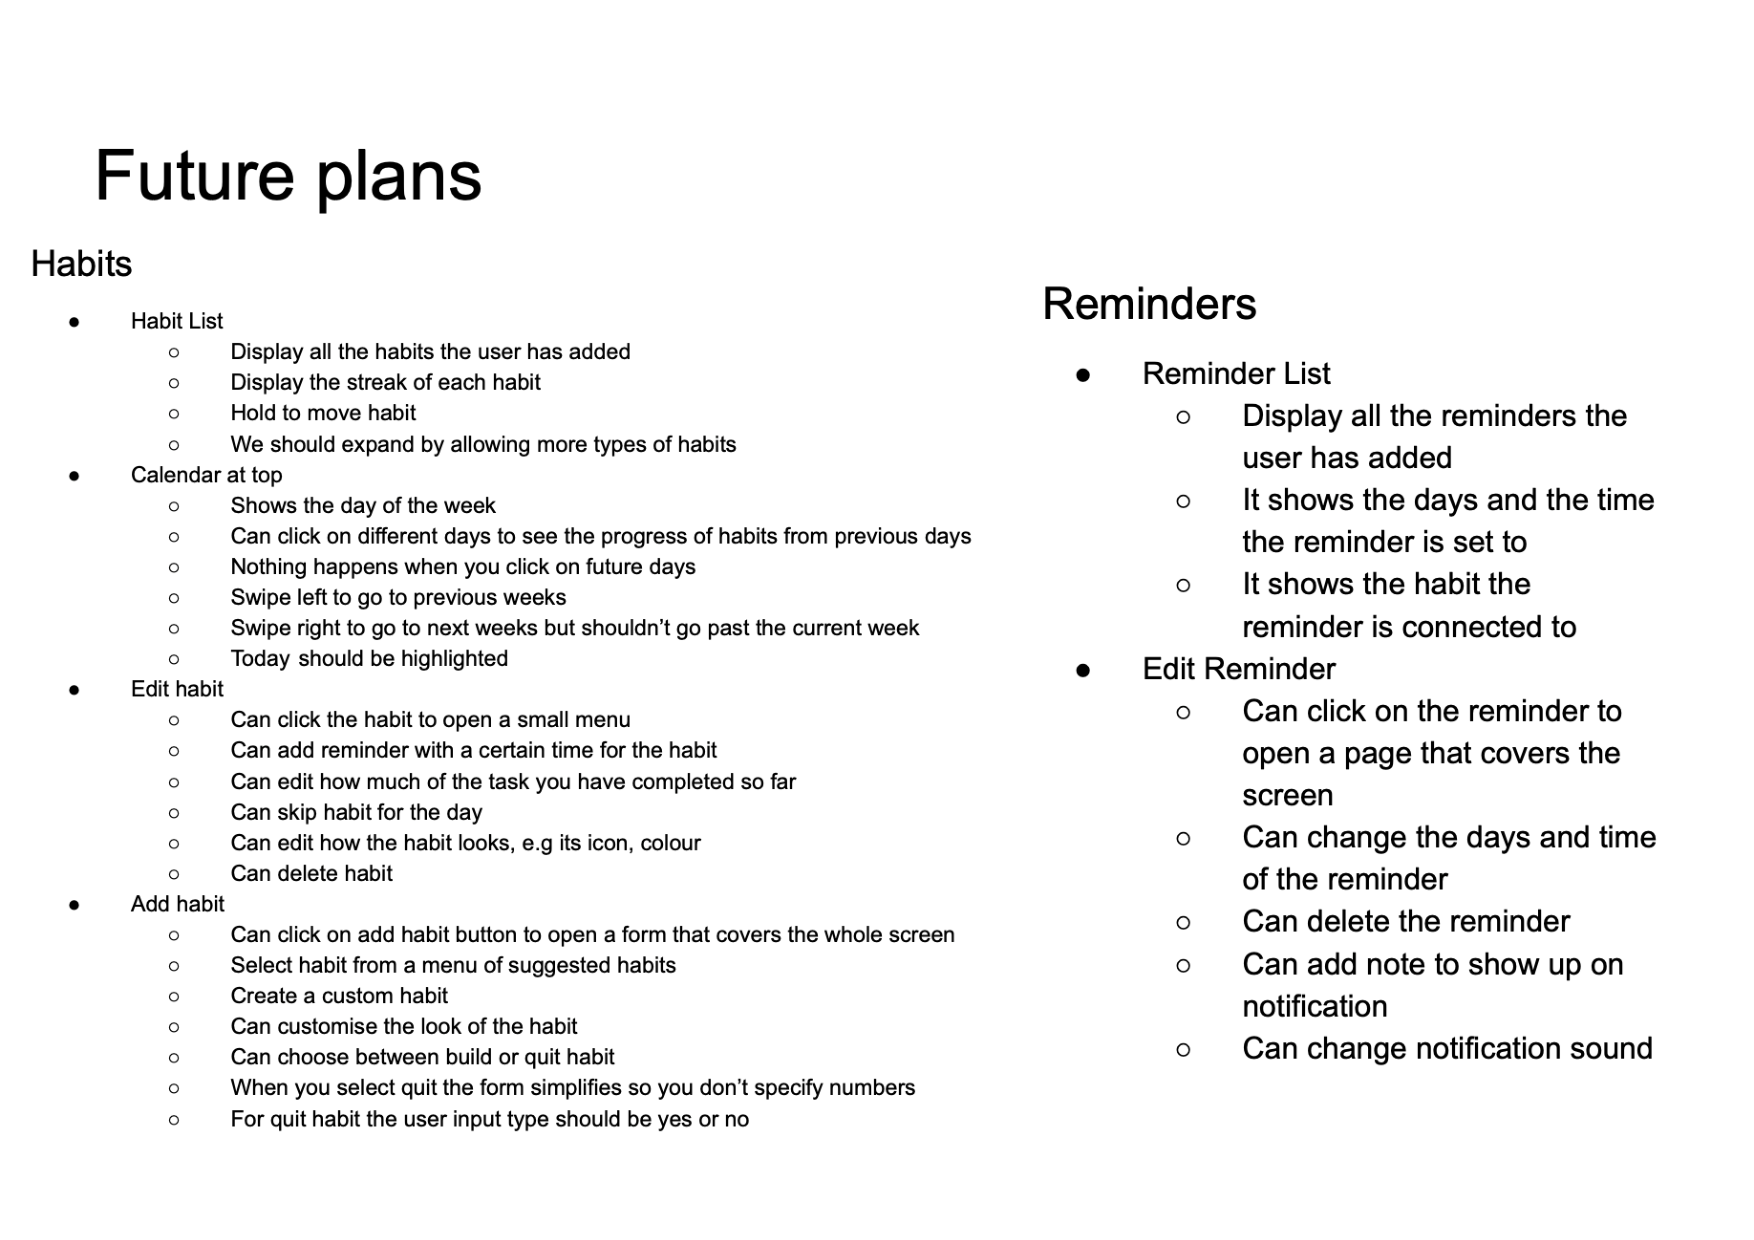
\includegraphics[width=0.7\textwidth]{resources/task_list.pdf}
    \caption{Page 1 of our backlog of organised tasks defined during the Week 2 Planning meeting (28/01/25)}
    \label{fig:task_list}
\end{figure}

\subsection{Communication Planning}
We formally agreed on the following communication strategies (as recorded in Team Feedback Meeting Minutes 29/01/25):

\begin{itemize}
    \item \textbf{Weekly Team Meetings:} Every Wednesday, in FWB Library.
    \begin{itemize}
        \item Discuss tasks completed, tasks in progress, and next steps.
    \end{itemize}
    \item \textbf{Online Communication (Discord):} For quick updates, online meetings, and working together on tasks.
    \item \textbf{Team Feedback \& GitHub Integration:} We used Team Feedback to share commits and attribute coding work. Collaborative coding sessions were recorded to ensure proper credit distribution.
\end{itemize}

One aspect of communication that we found effective and would implement again is the use of different communication channels on Discord. This allowed us to organise and manage our online discussions effectively, ensuring all saved materials were in one place and weekly targets were clearly communicated (see Figure \ref{fig:discord_channels}).

\begin{figure}[H]
    \centering
    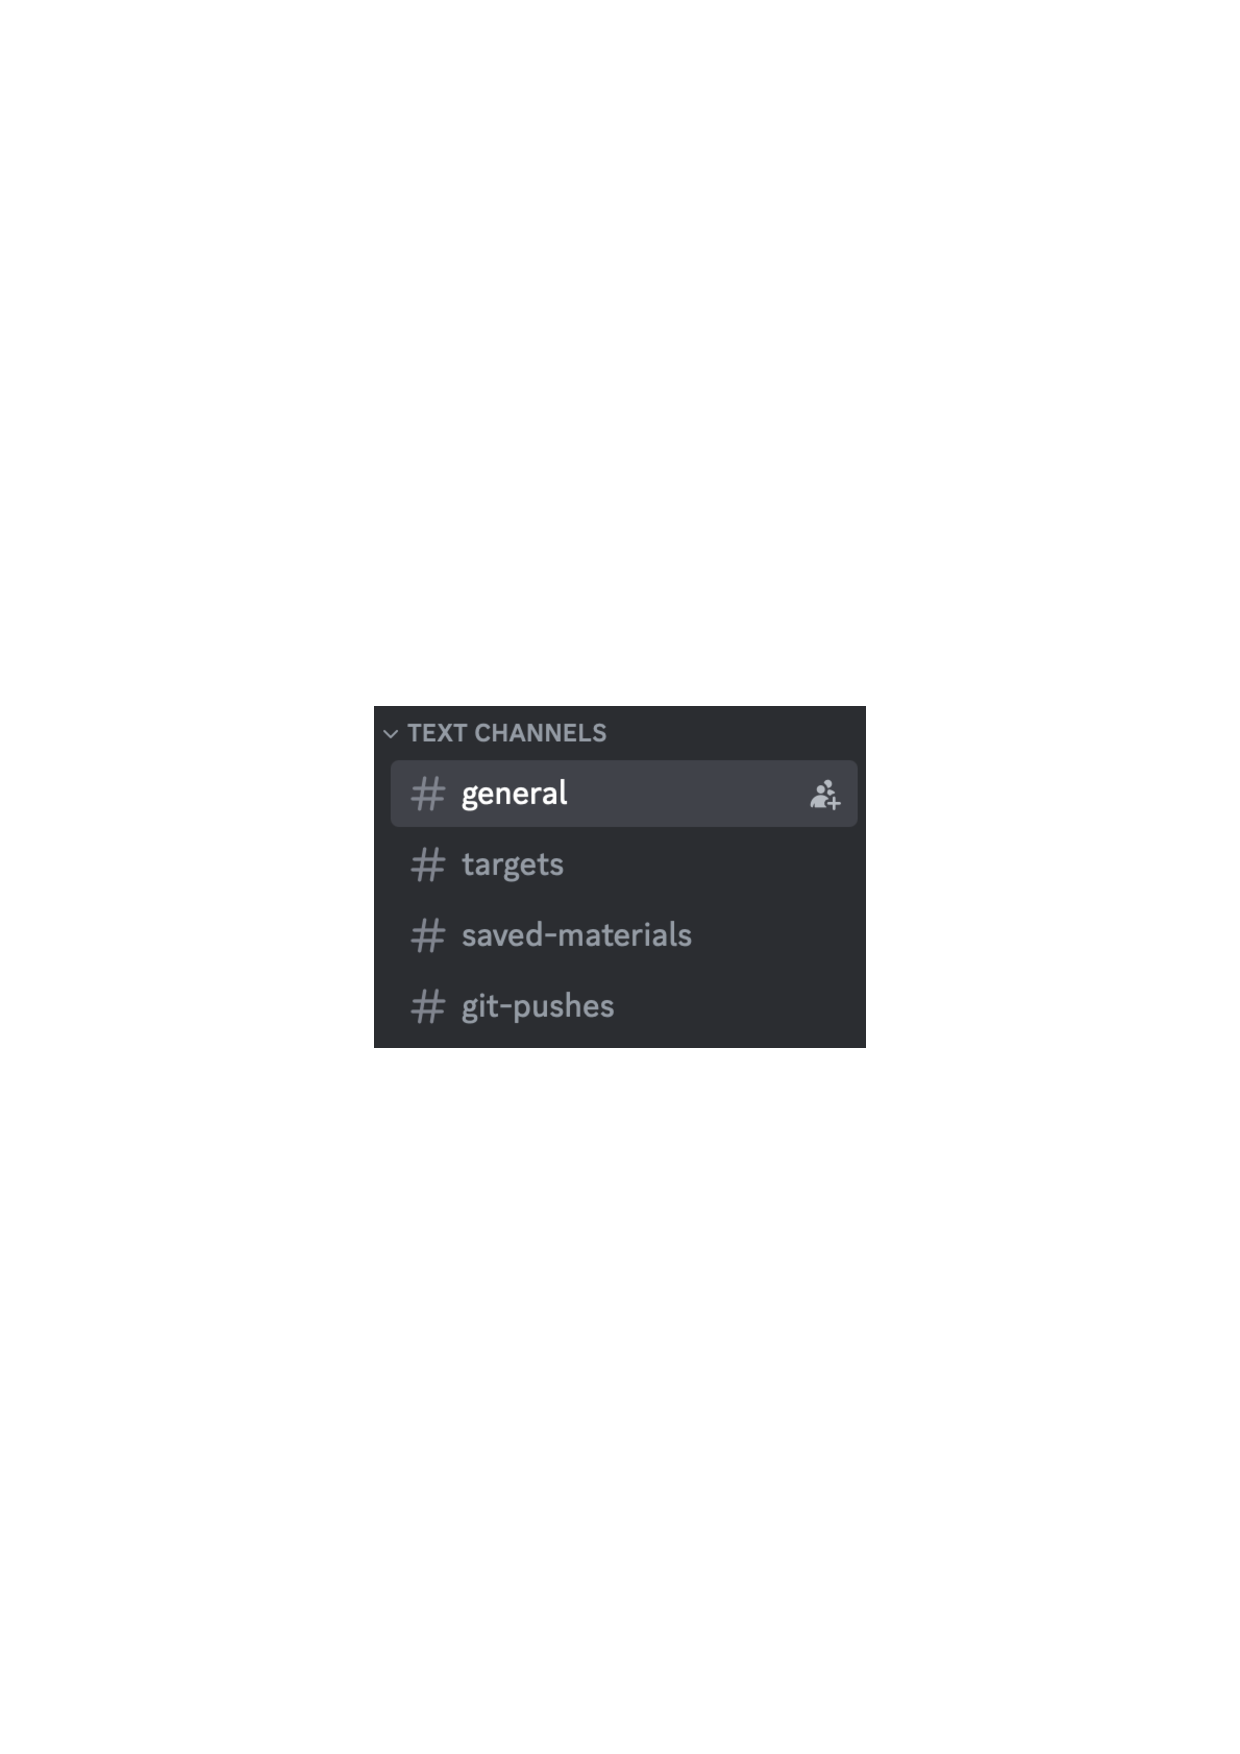
\includegraphics[width=0.7\textwidth]{resources/discord_channels.pdf}
    \caption{Different Discord communication channels used in the project}
    \label{fig:discord_channels}
\end{figure}

A critical reflection here is that, despite this plan, some members disengaged, which caused delays in certain tasks (see Section 4.2.2). This demonstrates how initial communication plans can be tested under real project conditions.

\section{Execution}
Execution involved turning our plans into tangible deliverables—writing code, creating the database structure, designing interfaces, and more.

\subsection{Task Allocation and Progress Tracking}
We adopted a weekly task allocation model at the start of each Wednesday meeting. For instance:
\begin{itemize}
    \item \textbf{Hugo:} Responsible for integrating new habit data into the MySQL database.
    \item \textbf{Doris:} Responsible for the statistics-page database functionalities.
\end{itemize}

Each person reported on progress the following week, as recorded in meeting minutes. If tasks were incomplete, we reassigned them or extended deadlines.

For evidence of this approach, see the weekly minutes excerpt below:

\begin{quote}
\textbf{Excerpt 4.1.} Individual accountability of task (Minutes 12/02/25)\\
\textit{"Action/commitment: Add selector to statistics page to pick different habits in the table.\\
Person responsible: Ming\\
Deadline: 12/02/25\\
Progress: In progress, deadline extended to 26/02/25"}
\end{quote}

This approach worked well, as it allowed us to keep track of individual progress, maintain accountability, and identify tasks requiring extra attention. In the future, we could enhance this method by including more detail in the ‘Progress’ section of our weekly minutes, requiring each member to specify exactly what was done. This would provide a deeper understanding of the development process.

\subsection{Dealing with Disengagement}
A challenge we faced was the partial disengagement of some team members, which manifested through missed meetings and uncompleted tasks. As recommended by agile methodologies \cite{schwaber2020scrum}:
\begin{itemize}
    \item We reassigned tasks when a member missed more than two consecutive meetings without prior notice.\\
    \textit{Example:} As recorded in Meeting Minutes 26/02/25, under New Commitments: “Reassigned calendar page task to Andrew.”
    \item We reduced the scope of certain features (e.g., scaled back the AI-based habit recommendation system).
\end{itemize}

\subsection{Ensuring Code Quality}
Initially, we planned code inspections and peer reviews for each major functionality. However, in practice:
\begin{itemize}
    \item We relied heavily on automated testing instead of thorough peer reviews.
    \item Due to time constraints, we conducted fewer formal inspections and prioritised feature completion.
\end{itemize}

In retrospect, while automated testing coverage was beneficial, face-to-face reviews could have caught inconsistencies earlier. This aligns with standard software engineering advice, which highlights that code reviews often catch design and logic flaws beyond what unit tests detect \cite{fowler2018refactoring}.

\section{Monitoring and Control}
Monitoring and control involved continuously checking our progress against the plan and adapting as needed.

\subsection{Regular Check-ins and Task Status}
Each weekly meeting served as a control point:
\begin{itemize}
    \item We reviewed completed tasks vs. planned tasks.
    \item We updated the Trello board (e.g., moving items to “Done” or reassigning them).
    \item We merged completed branches to the master branch on GitHub together, preventing serious conflicts.
\end{itemize}

\begin{figure}[H]
    \centering
    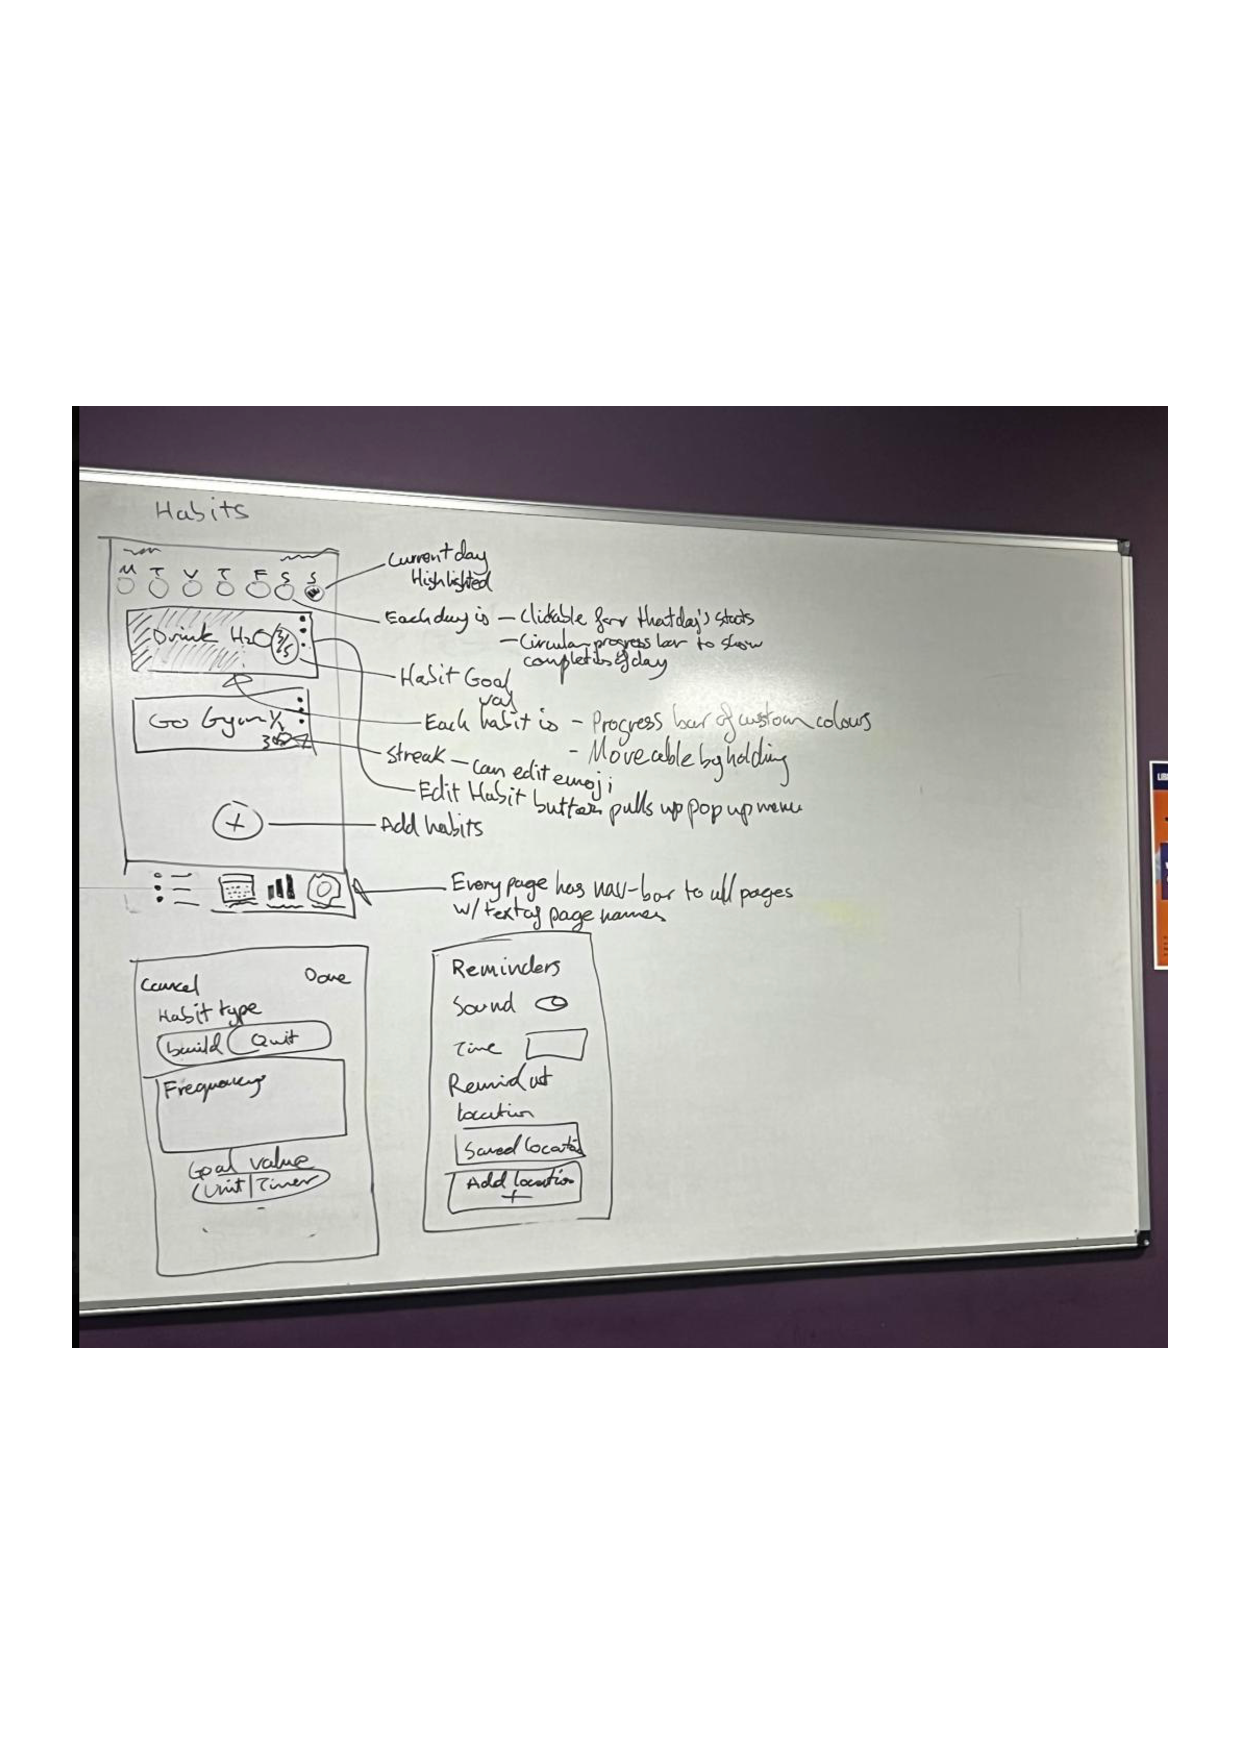
\includegraphics[width=0.7\textwidth]{resources/board.pdf}
    \caption{Designing the app during a weekly meeting}
    \label{fig:whiteboard_meeting}
\end{figure}

We conducted a project review meeting where we reassessed project risks, scheduling, and communication plans (Meeting Minutes 26/02/25). A key issue we identified was that we only held one project review meeting, which we believe was insufficient for a project of this duration. 

\section{Close}
Finally, closing the project required delivering the final software product and supporting materials.

\subsection{Preparing Final Deliverables}
\begin{itemize}
    \item \textbf{Codebase:} Fully merged into the main branch on GitHub.
    \item \textbf{App Deployment:} Tested on Expo Go for iOS and verified basic web accessibility.
    \item \textbf{Test Deployments:} Conducted in a staging environment.
\end{itemize}

\section{Conclusion}
Our hybrid Agile/Waterfall approach provided structure and flexibility. Despite challenges, we successfully adapted by reallocating tasks, adjusting our scope, and focusing on core deliverables.





